\newcommand{\institut}{}
\newcommand{\fachgebiet}{Halbleiterbauelemente}
\newcommand{\veranstaltung}{Praktikum Technologie und Bauelemente der Halbleitertechnik}
\newcommand{\pdfautor}{Dirk Barbendererde (321 836), Thomas Kapa (), Alona
Siebert (), Özgü Dogan (326048)}
\newcommand{\autor}{Dirk Barbendererde (321 836)\\ Thomas Kapa ()\\ Alona
Siebert ()\\ Özgü Dogan (326 048)}
\newcommand{\pdftitle}{Praktikum\ Technologie und Bauelemente der
Halbleitertechnik}
\newcommand{\prototitle}{Praktikum Technologie und Bauelemente der Halbleitertechnik}
\newcommand{\aufgabe}{}

\newcommand{\gruppe}{Gruppe 1}
\newcommand{\betreuer}{Betreuer:\\ Clemens Helfmeier\\ Philipp Scholz}



\input{../../packages/tu_header_9}

\setcaptionwidth{7.5cm}

\begin{document}


%     \lstinputlisting{./praktikum6.sce}



%---------------------------------------------------------------------
%---------------------------------------------------------------------
%---------------------------------------------------------------------

\section{Kennlinie}
\begin{quote}
    
    Benennung der Dateien:\\
    Kennlinie_{Wavernummer}_Die_[{Zeile},{Spalte}]_Mess_{messung}.mat\\
    
    100 µA Strombegrenzung\\
    Welche Diode?
    Welcher Manipulator
    
    SMU1 = GND
    SMU2 = GND
    SMU3 = Var1
    
    Unterdiffusion
    
    unterspannung
    0.0 & 2.4
    0.5 & 3.8
    0.8 & 4.5
    1.0 & 5.0
    1.3 & 5.5
    1.8 & 6.7
    2.5 & 8.2
    3.0 & 9.2
    
    \TODO{müssen wir die Dies durchnummerieren?}
\end{quote} %sec Kennlinie

%--------------------------------------------------------------------
%--------------------------------------------------------------------

\section{Schaltverhalten}
\begin{quote}
    
\end{quote} %sec Schaltverhalten

%--------------------------------------------------------------------
%--------------------------------------------------------------------

\section{Emissionsmessung}
\begin{quote}
    
    \TODO{Einleitung, Theorie, Verknüpfung, Messung, Ergebnisse, Auswertung}
    
    Eine Emissionsmessung ist in der Halbleitertechnologie insofern interessant,
    weil sie Erkenntnisse über charakteristische Eigenschaften des Halbleiters,
    in unserem Fall die selbst hergestellte Diode, liefert. Dazu gehören die
    Ladungsträgerlebensdauer $\tau_{n,p}$ und die Diffusionslänge $L_{n,p}$. Auf
    die Lebensdauer lässt sich mithilfe der Diffusionslänge und des
    Diffusionskoeffizienten schließen. Dieser ist ein materialabhängiger Wert,
    welcher von uns nicht weiter beachtet wird. Der folgende Zusammenhang hilft
    bei der Berechnung von $\tau_{n,p}$:
    
    \begin{equation*}
        \begin{split}
            L_{n,p} = \sqrt{\tau_{n,p} \cdot D_{n,p}} 
        \end{split}
    \end{equation*}
    
    Ziel unserer Messung aber war die Bestimmung der Diffusionslänge in unserer
    Diode. Dieser wurde über die realisierte Intensitätsmessung anhand der
    Emissionen in der Diode ermittelt. Dabei wurden folgende
    Proportionalitätsverhätnisse verwendet:
    
    \begin{equation*}
        \begin{split}
            I(x) \sim \ \Delta n \sim \ exp(-\frac{x}{L_n}) 
        \end{split}
    \end{equation*}
    
    Hierbei werden Strahlungsintensität ins Verhältnis mit der\\
    Minoritätsüberschussladungträgerkonzentration und dieser wiederum 
    ins Verhältnis mit einem Exponentialtherm gesetzt. Daher kann man die
    Intensitätsmessung direkt mit diesem Therm in Verbindung setzen, 
    welcher in seinem Argument die gesuchte Diffusionslänge beinhaltet. Weiteres
    zur Berechnung des $L_n$ steht in der Auswertung der Messung.\\
    
    Um aber die Intensitätsmessung verstehen zu können müssen einige
    grundlegende Theorien der Halbleiter bezüglich ihrer Typen und ihrer
    Rekombinationsarten behandelt und nachvollzogen werden.\\ 
    Daher gibt es vor der Versuchsdurchführung und der Auswertung zunächst eine
    kleine Exkursion in den theoretischen Bereich.
    
        \subsection{Direkter und indirekter Halbleiter }
        \begin{quote}
        
        Es gibt zwei Arten von Halbleitern, die direkten und die indirekten
        Halbleiter. Diese unterscheiden sich darin, dass die Rekombination eines
        Ladungsträgers aus dem Leitungs- in das Valenzband unterschiedliche
        Vorraussetzungen erfordert.
            
            \subsubsection{direkter Halbleiter}
            \begin{quote}
            Die Rekombination bei einem direkten Halbleiter ist relativ simpel.
            Ein freies Elektron braucht dabei nur, unter Abgabe der jeweiligen
            Energie, den Bandabstand zwischen Leitungs- und Valenzband zu
            überqueren.
            
            \begin{figure}[H]
                    \centering
                        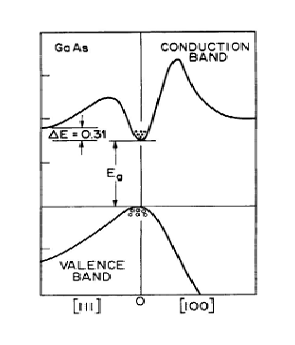
\includegraphics[scale=0.72, trim = 1cm 0cm 1.5cm 0cm,
                        clip]{./Emissionsbilder/restliches/direkt.png}
                        \caption{Rekombination bei einem direkten Halbleiter}
                            \label{fig:./Emissionsbilder/restliches/direkt.png}
            \end{figure}
            
            
            \end{quote}       
        
            \subsubsection{indirekter Halbleiter}
            \begin{quote}
            Die Rekombination bei einem indirekten Halbleiter erfordert neben
            einem Energieunterschied auch einen Impulsunterschied, damit das
            Elektron auf dem Valenzband auftreffen kann. Dieser
            Impulsunterschied ist in der folgenden Abbildung zu erkennen.
            
            \begin{figure}[H]
                    \centering
                        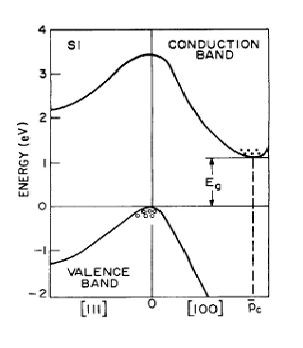
\includegraphics[scale=0.73, trim = 1cm 0cm 1.5cm 0cm,
                        clip]{./Emissionsbilder/restliches/indirekt.png}
                        \caption{Rekombination bei einem indirekten Halbleiter}
                            \label{fig:./Emissionsbilder/restliches/indirekt.png}
            \end{figure}
            
            \TODO{Bildquellen, TBH-Skript S.92 einfügen}
            \end{quote}       
            
            Ein weiterer Unterschied zwischen direkten und indirekten
            Halbleitern ist der, dass direkte Halbleiter hauptsächlich
            strahlend rekombinieren, wohingegen indirekte Halbleiter
            stochastisch betrachtet fast nur nichtstrahlend rekombinieren.
            Dennoch findet mit sehr geringer Wahrscheinlichkeit auch vereinzelt
            strahlende Rekombination in den indirekten Halbleitern statt.\\
            Bevor weiter darauf eingegangen wird, in wie fern dies für die
            Emissionsmessung von Bedeutung ist, werden die Rekombinationsarten,
            strahlend und nichtstrahlend, wiederholt.
            
        \end{quote}
        
        \subsection{Rekombinationsmechanismen}
        \begin{quote}
        
        Eine Rekombination erfolgt stets unter Abgabe von einer
        Energiedifferenz. Dabei wird unterschieden, ob diese Energie in Form
        eines Lichtquants oder von Wärme abgegeben wird, wodurch auch die
        Beschreibung strahlend oder nichtstrahlend entsteht.\\
        Nun folgen je ein Beispiel für diese Machanismen.
        
            \subsubsection{strahlende Rekombination}
            \begin{quote}
            
            Die strahlende Rekombination, hauptsächlich bei direkten Halbleitern
            zu sehen, besagt, dass der rekombinierende Ladungsträger die
            Energiedifferenz, welche er zurücklegt, in Form eines Photons
            freigibt. Die Energie dieses Photons beträgt genau die Energie des
            Bandabstands zwischen den beiden Bändern. Anders ausgedrückt kann
            man sie auch Rekombinationsenergie nennen:
                    
            \begin{equation*}
                \begin{split}
                    W_{Rek} = h \cdot \nu 
                \end{split}
            \end{equation*}
            
            Diese Rekombinationsenergie setzt sich aus des Produkt aus dem
            Planckschen Wirkungsquantums $h$ und die Frequenz des entstehenden
            Lichts $\nu$.\\
            
            Ein Beispiel für die strahlende Rekombination ist die
            Band-Band-Rekombination, welche in der folgenden Abbildung
            dargestellt wurde:
            
            \begin{figure}[H]
                    \centering
                        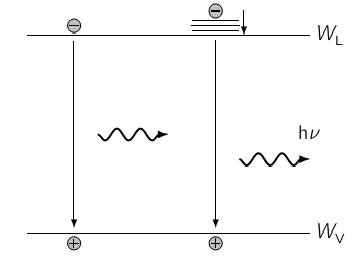
\includegraphics[scale=0.72, trim = 1cm 0cm 1.5cm 0cm,
                        clip]{./Emissionsbilder/restliches/bandband.png}
                        \caption{strahlende Band-Band-Rekombination}
                            \label{fig:./Emissionsbilder/restliches/direkt.png}
            \end{figure}
            
            Man erkennt ein Elektron, welches beim Rekombinieren, die bereits
            erwähnte Rekombinationsernergie in Form eines Photons abgibt. Es
            kann aber auch vorkommen, dass die abgegebene Energie an ein
            weiteres Eektron im Leitungsband abgegeben wird, wodurch dieser auf
            ein höheres Energieniveau im Leitungsband angehoben und wieder runterfallen 
            kann. Diese Möglichkeit ist bei der strahlenden Rekombination die
            unwarscheinlichere Variante.
            
            \end{quote}
            
            \subsubsection{nichtstrahlende Rekombination}
            \begin{quote}
            
            Die nichtstrahlende Rekombination findet hauptsächlich bei
            indirekten Halbleitern statt. Dabei wird die Rekombinationsenergie
            an ein weiteres Elektron im Leitungsband abgegeben, welches auf ein
            höheres Energieniveau angehoben wird und unter Abgabe von
            thermischer Energie wieder runterfallen kann.\\
            Als ein Beispiel für die nichtstrahlende Rekombination wird die
            Augerrekombination dargestellt:
            
            \begin{figure}[H]
                    \centering
                        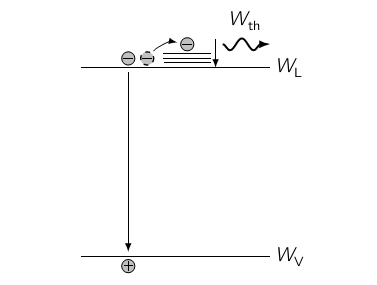
\includegraphics[scale=0.72, trim = 1cm 0cm 1.5cm 0cm,
                        clip]{./Emissionsbilder/restliches/auger.png}
                        \caption{nichtstrahlende Auger-Rekombination}
                            \label{fig:./Emissionsbilder/restliches/auger.png}
            \end{figure}
            
            \TODO{Bildquellen einfügen: TBH-Skript S.93,94}
            \end{quote}
        
        Die für die Emissiosmessung verwendete Diode besteht aus Silizium,
        welcher ein indirekter Halbleiter ist und dessen Rekombinationen
        hauptsächlch nichtstrahlend sind. Wie aber schon bei den Halbleitertypen
        erwähnt, kann es bei indirekten Halbleitern auch mit sehr geringer
        Wahrscheinlichkeit zu strahlender Rekombination kommen. Da die Abgabe
        von thermischer Energie zu einem Temperaturunterschied in der Diode
        führen würde, bräuchte man bei den Emissionsmessung sehr feine und genau
        Thermometer, welche im $\mu m$-Bereich nicht realisierbar sind. Daher
        wird die stochastisch in geringer Menge vorhandene strahlende
        Rekombination betrachtet um über die mit lichtempfindlichen
        Kameras gemessene Lichtintensitäten auf die gesuchte Diffusionslänge
        schließen zu können.
        
        \end{quote}
        
        \vspace{1.5em}
        
        Emission entsteht bei der Rekombination eines freien Ladungsträgers,
        welches nur in Durchlassrichtung bei einer Diode erwartet wird. Dabei
        werden die Majoritäten ins entgegen gesetztes Gebiet injeziert und
        rekombinieren dort als Minoritäten mit den oppositär gepolten
        Ladungsträgern. Die dabei freigesetzte Energie kann dann als Emission
        wargenommen werden. Emission kann aber auch in Sperrrichtung entstehen.
        Die sogennante Feldemission findet dabei ausschließlich in der
        ausgebreiteten Raumladungszone statt. Sobald eine Sperrspannung an der
        Diode angelegt wird, werden die freien Ladungsträger aus der
        Raumladungszone gesaugt und erfahren dabei eine kinetische Energie,
        dessen Stärke von der Größe der Sperrspannung abhängt. Während der
        beschleunigten Bewegung der Ladungsträger aus der Raumladungszone,
        können diese mit Gitteratomen zusammenprallen und Elektronen aus diesem
        Atom auf ein höheres Energieniveau anheben. Wie bei der nichtstrahlenden
        Rekombination entsteht bei diesem Vorfall hauptsächlich thermische
        Energie,es kann aber auch, mit einer sehr kleinen wahrscheinlichkeit
        eine strahlende Rekombination vorkommen.\\
        Die Feldemission ist im Vergleich zu der Emission in Flussrichtung
        unbedeutend klein. Daher ist für die Intensitätsmessung nur eine
        Emission in Flussrichtung relevant.
        
        \vspace{1.5em}
        
        \subsection{Messaufbau}
        \begin{quote}
        
        Die Emissionsmessung erfolgt, wie in der Einleitung erwähnt, durch eine
        Intensitätsmessung während der Rekombinationen in Flussrichtung der
        Diode. Die Messung wird mithilfe des Phemos 1000 durchgeführt, welches
        ein Prüfgerät in der Halbleitertechnik ist und hauptsächlich für
        Fehlerdetektion dient. Um diese geringe Lichtintensität
        messen zu können, braucht man eine lichtempfindliche CCD Kamera. Diese
        ist im Phemos integriert und muss während der gesamten Messung auf
        $-50$°C gekühlt werden. So werden thermische Rauscheinflüsse der sehr 
        empfindlichen Kamera vermieden um das Ergebnis nicht zu verfälschen.\\
        
        Der Wafer, mit mehreren Diodenstrukturen, wird in dem Innenraum des
        Phemos auf einer Vakuumplatte fixiert, sodass der erwünschte Bereich des
        Wafers mit dem passenden Objektiv vergrössert werden kann. Diese
        Vergrößerung hilft bei der Kontaktierung des p- und des n-Pads der Diode
        anhand Nadelspitzen, welche in der unteren Abbildung im Licht des
        Mikroskops zu erkennen sind.
        
        \begin{center}
                \begin{tabular}{ll}
    
                \hspace{-8em}
                    \begin{minipage}{0.6\textwidth}
    
                        \begin{figure}[H]
                            \label{fig:}
                            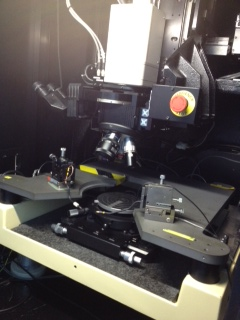
\includegraphics[scale=0.7, trim = 0cm 0cm 0cm
                            0cm, clip]{./Emissionsbilder/restliches/phemos1.JPG}
                            %FIXME [width=640px,
                             %height=474px]
                            \caption{Innenraum des Phemos}
                        \end{figure}
    
                    \end{minipage}
                    \begin{minipage}{0.6\textwidth}
    
                        \begin{figure}[H]
                            \label{fig:}
                            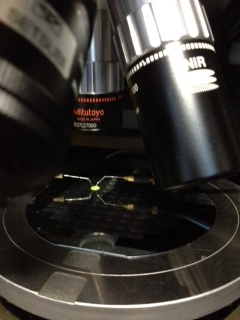
\includegraphics[scale=0.7, trim = 0cm 0cm 0cm
                            0cm, clip]{./Emissionsbilder/restliches/phemos2.JPG}
                            %FIXME [width=640px,
                             %height=474px]
                            \caption{kontaktierte Diode auf dem Wafer}
                        \end{figure}
                    \vspace{-1.5em}
    
                    \end{minipage}
    
                \end{tabular}
                \end{center}
        
        \vspace{2em}
        
        Anhand eines Live-Bilds der CCD Kamera, kann man bis zum Start der
        Messung den fokussierten Bereich bepannungsquelle für den
        Durchlassbetrieb der Diode wurde der HP4145A, ein sensibeles
        Analysegerät für Halbleiterbauelemente, verwendet, mit welchem eine
        konstante Spannung für eine einstellbare Zeitspanne eingestellt werden
        kann. Somit konnte man fest davon ausgehen, dass die Diode ohne einen
        Spannungseinbruch konstant in Durchlassrichtung betrieben wurde.\\
        Die Messdauer der Emission wurde mithilfe der Phemos-Software
        eingestellt. Mit welchen Durchlassspannungen und wie lange gemessen
        wurde, wird in der Auswertung der Messergebnisse angegeben.\\
        Am Ende jeder Messung wurde noch eine Dark-Substraction durchgeführt.
        Bei dieser Dark-Substraction wird die Durchlassspannung abgeschaltet,
        wodurch die Diode nicht mehr als aktiv betrachtet wird. Die Emissionsmessung wird mit der
        gleichen Messdauer und deaktivierter Diode nochmal durchgeführt und von
        der eigentlichen Emissionsmessung subtrahiert, damit jegliche
        Rauscheinflüsse des Phemos selbst aus den Messergebnissen ausgeschlossen
        werden können. 
        
        \end{quote}
        
        \subsection{Messergebnisse}
        \begin{quote}
        
        Die Active-Area- und Kontaktfenstermasken wurden so erstellt, dass der
        Wafer am Ende der Produktion Dioden auf jedem Die besaß, die für diese
        Emissionsmessung hergestellt wurden. Diese hatten die Besonderheit, dass
        zwischen p- und n-Pad das Substrat nicht mit Siliziumoxid beschichtet
        war, damit an den pn-Übergang zwischen n-Gebiet und p-Substrat
        unverfälschte Emission gemessen werden konnte. Man hätte annehmen
        können, dass dort, wo Oxid auf dem pn-Übergang lag, keine Emission aus
        dem Wafer austreten und gemessen werden kann. Die Praxis bewies aber das
        Gegenteil. Unabhängig von der Auswertung der Messung
        konnte an den pn-Übergängen mit Siliziumoxid darüber eine viel stärkere
        Emission gemessen werden. Der Grund dafür lag in dem Brechungsindex und
        der Dicke der Oxidschicht, denn durch die Reflexionen der Strahlung an
        den Übergängen von Silizium zu Siliziumoxid und Siliziumoxid zur Luft
        wurden die Strahlen so reflektiert, dass konstruktive Interferenz
        zwischen den Lichtwellen entstand und somit die Emission als viel
        stärker wahrgenommen wurde. Da dies nicht die wirkliche Intensität der
        Emission am pn-Übergang unserer Diode wiederspiegelt, wurden diese mit
        Oxid überlagerten Stellen in der Emissionsmessung vernachlässigt.\\
        
        Gemessen wurde nur der Bereich von der Grenze des n-Gebiets bis in
        das p-Substrat hinein. Als Hilfe dafür wurde das jeweilige Emissionsbild
        der Phemos-Software verwendet. Diese zeigte mit farblichen Unterschieden
        (rot = starke Emission, blau = schwache Emission) wo der sinnvolle
        Messbereich begann und endete. Die folgenden Abbildungen zeigen die
        Diode vor und nach der Emissionsmessung auf dem Die in Zeile $6$ und
        Spalte $3$ des Wafers. Zunächst wurde eine große, dann eine kleinere
        Emissions-Diode ausgemessen. Bei beiden betrug die Durchlassspannung
        $1,2 V$ bei $25 mA$ und einer Messdauer von $4s$.
        
         \begin{center}
                \begin{tabular}{ll}
    
                \hspace{-10em}
                    \begin{minipage}{0.6\textwidth}
    
                        \begin{figure}[H]
                            \label{fig:}
                            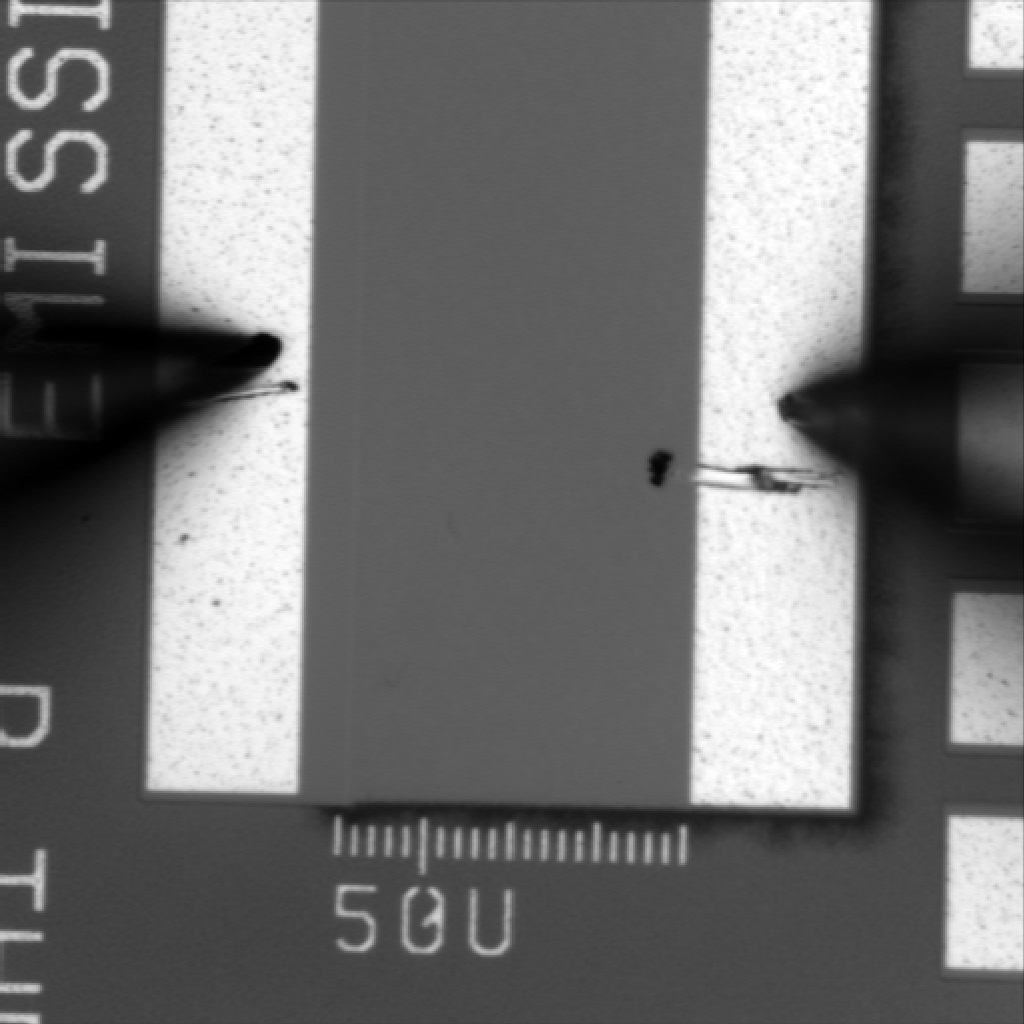
\includegraphics[scale=0.25, trim = 0cm 0cm 0cm
                            0cm,
                            clip]{./Emissionsbilder/eins/nach_Kontaktierung_vorMessung.jpg}
                            %FIXME [width=640px, height=474px]
                            \caption{kontaktierte Diode, Live-Bild der CCD
                            Kamera}
                        \end{figure}
    
                    \end{minipage}
                    \begin{minipage}{0.6\textwidth}
    
                         \begin{figure}[H]
                            \label{fig:}
                            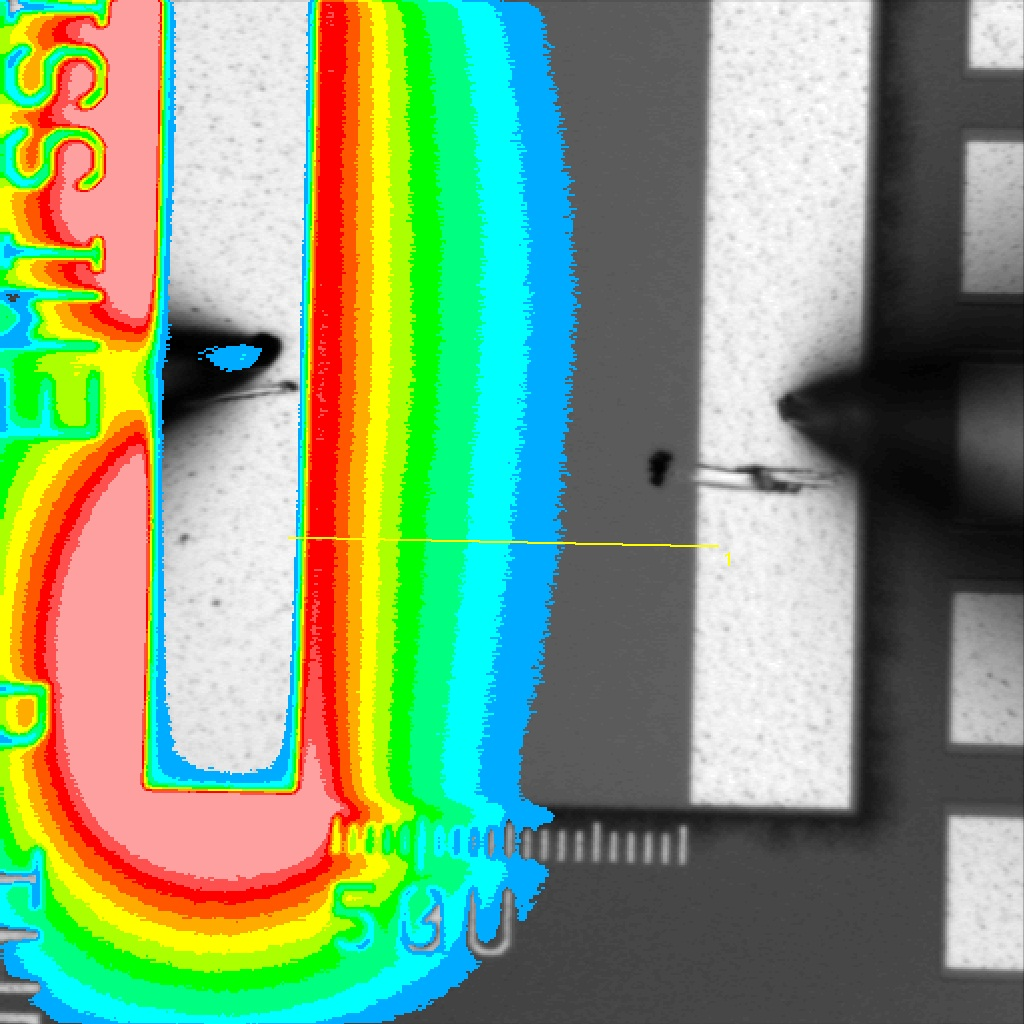
\includegraphics[scale=0.25, trim = 0cm 0cm 0cm
                            0cm,
                            clip]{./Emissionsbilder/eins/nach_Emission_mit_Distanzen.jpg}
                            %FIXME [width=640px, height=474px]
                            \caption{selbe Diode nach der Emissionsmessung}
                        \end{figure}
                   \vspace{-1.5em}
    
                    \end{minipage}
    
                \end{tabular}
                \end{center}
                
        \vspace{2em}
        
        Der gelbe Strich wurde anhand der Maus gezogen und zeigt den Bereich im
        Substrat, welcher genauer ausgewertet wurde. Mehr dazu folgt in der
        Auswertung.\\
        
        Als nächstes folgen die Abbildungen der kleineren Emissions-Diode auf
        dem selben Die:
             
        
         \begin{center}
                \begin{tabular}{ll}
    
                \hspace{-10em}
                    \begin{minipage}{0.6\textwidth}
    
                        \begin{figure}[H]
                            \label{fig:}
                            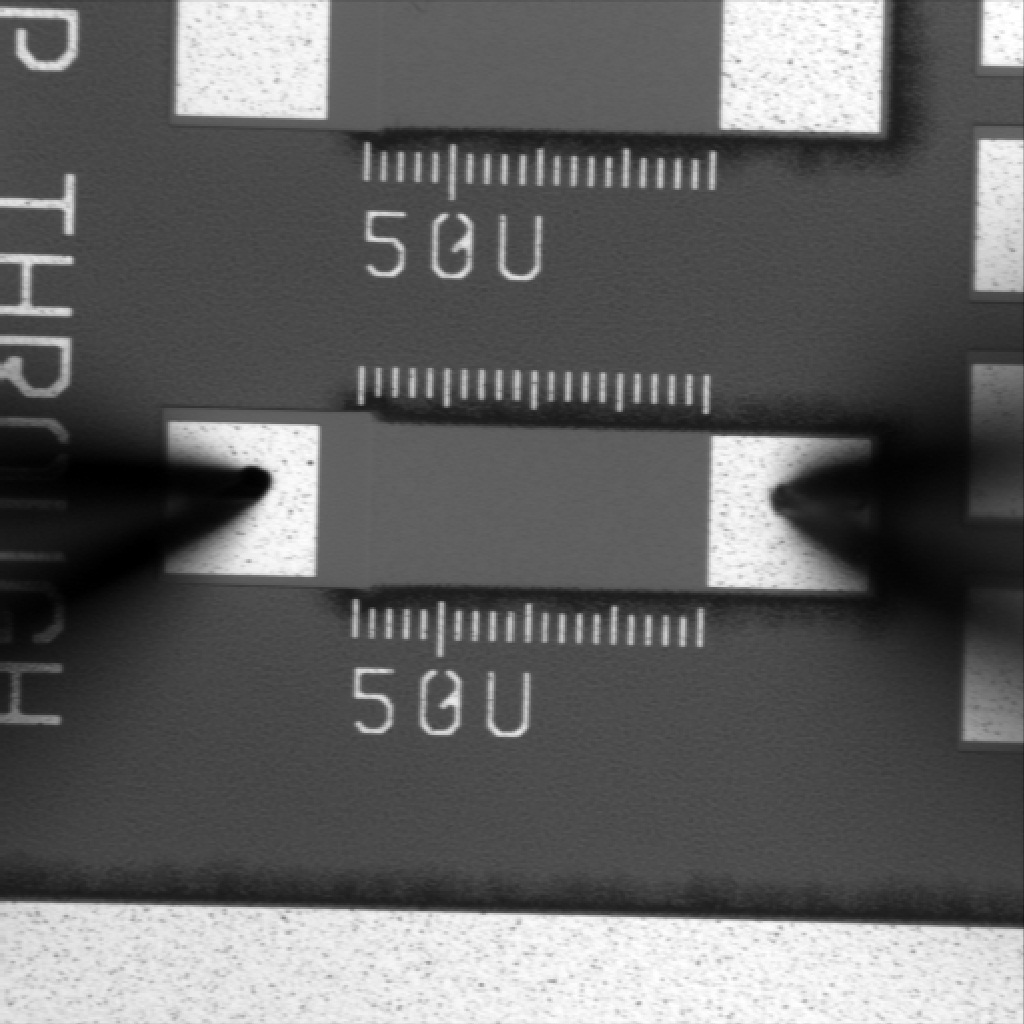
\includegraphics[scale=0.25, trim = 0cm 0cm 0cm
                            0cm,
                            clip]{./Emissionsbilder/zwei/nack_Kontaktierung.jpg}
                            %FIXME [width=640px, height=474px]
                            \caption{kontaktierte Diode, Live-Bild der CCD
                            Kamera}
                        \end{figure}
    
                    \end{minipage}
                    \begin{minipage}{0.6\textwidth}
    
                         \begin{figure}[H]
                            \label{fig:}
                            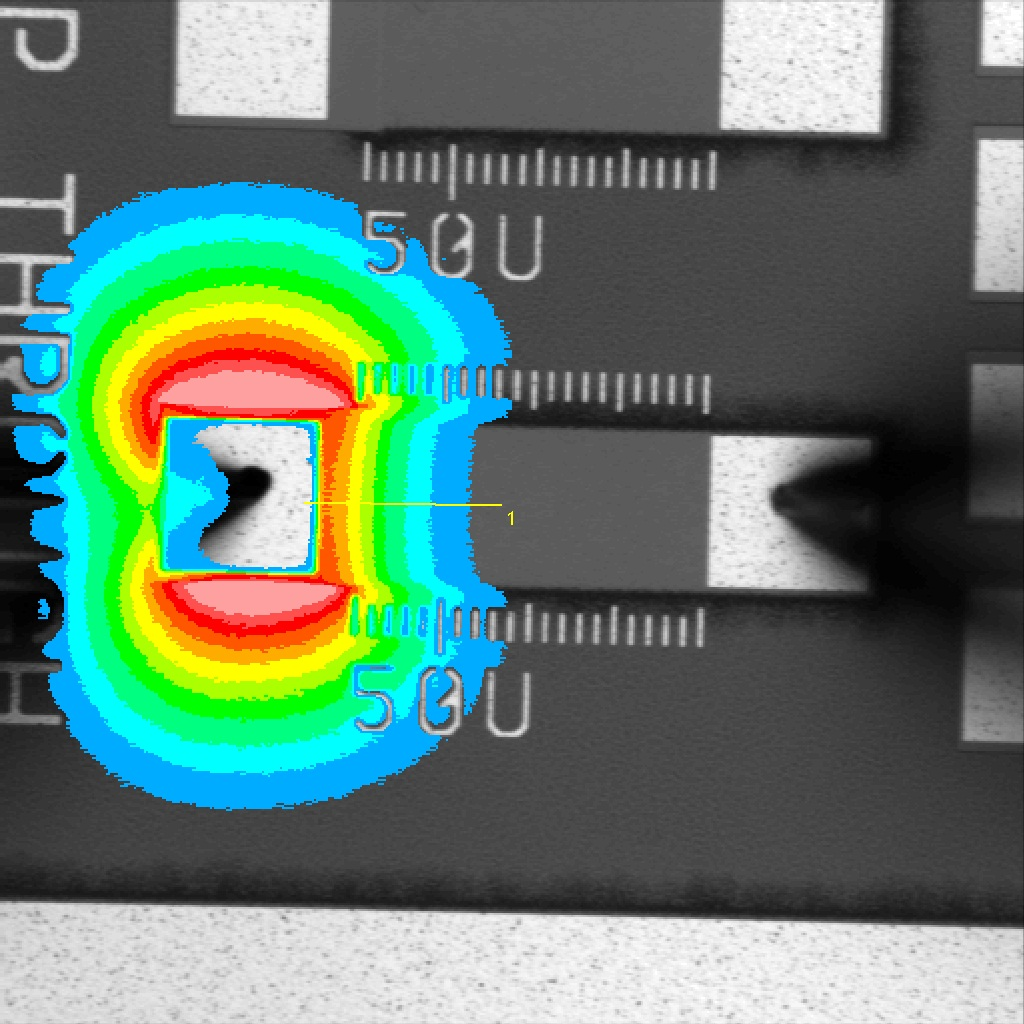
\includegraphics[scale=0.25, trim = 0cm 0cm 0cm
                            0cm,
                            clip]{./Emissionsbilder/zwei/nach_Emissionsmessung_Intensitat_Distanz.jpg}
                            %FIXME [width=640px, height=474px]
                            \caption{selbe Diode nach der Emissionsmessung}
                        \end{figure}
                   \vspace{-1.5em}
    
                    \end{minipage}
    
                \end{tabular}
                \end{center}
                
        \vspace{2em}
        
        Nun wurde noch ein Die am Rand des Wafers ausgemessen um nach
        Unterschieden zwischen den Messergebnissen kontrolliert werden zu
        können. Auch auf dem Die in Zeile $15$ und Spalte $8$ wurde erst eine
        große, dann eine kleine Emissions-Diode untersucht. Die Durchlassspannung bei der
        großen Diode betrug $1,2 V$ bei einem Strom von $25 mA$. Die Messdauer
        wurde aus $3s$ variiert.
        
        
         \begin{center}
                \begin{tabular}{ll}
    
                \hspace{-10em}
                    \begin{minipage}{0.6\textwidth}
    
                        \begin{figure}[H]
                            \label{fig:}
                            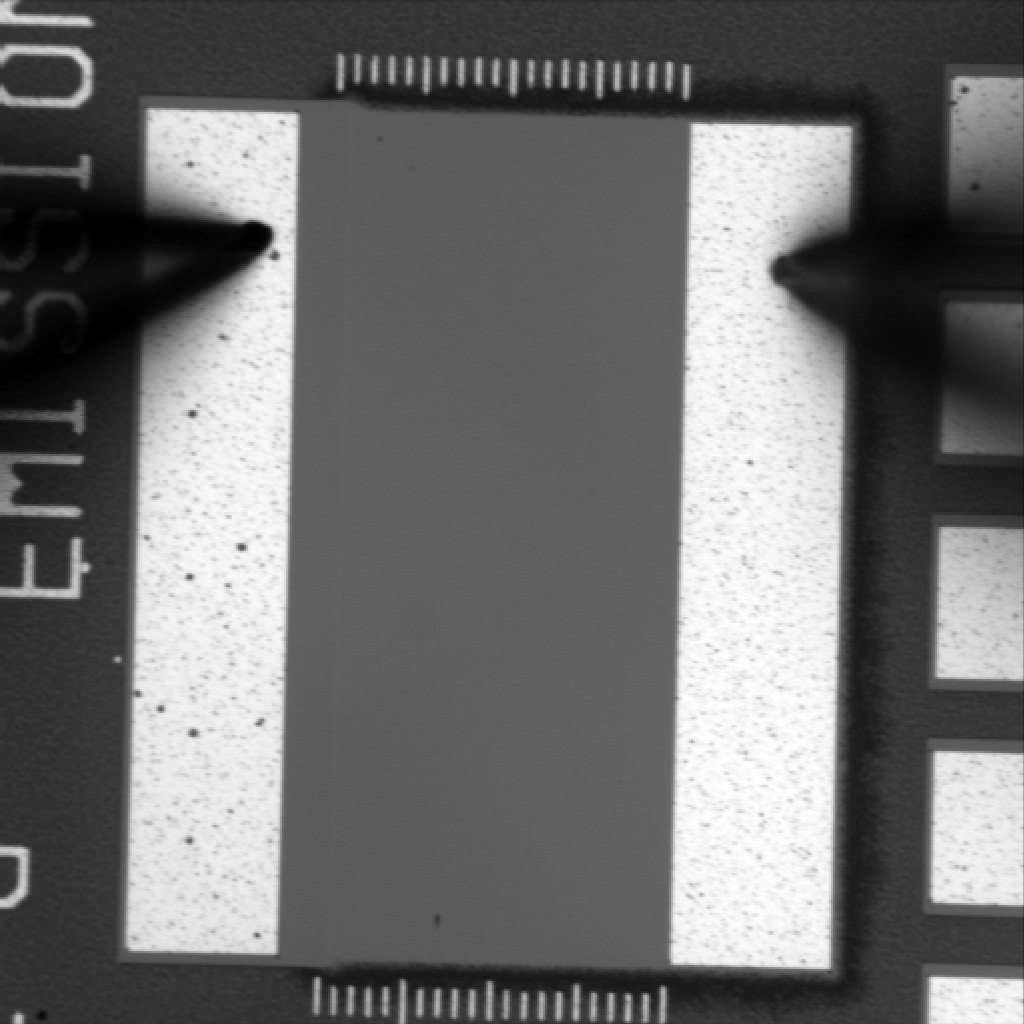
\includegraphics[scale=0.25, trim = 0cm 0cm 0cm
                            0cm,
                            clip]{./Emissionsbilder/drei/nach_Kontaktierung.jpg}
                            %FIXME [width=640px, height=474px]
                            \caption{kontaktierte Diode, Live-Bild der CCD
                            Kamera}
                        \end{figure}
    
                    \end{minipage}
                    \begin{minipage}{0.6\textwidth}
    
                         \begin{figure}[H]
                            \label{fig:}
                            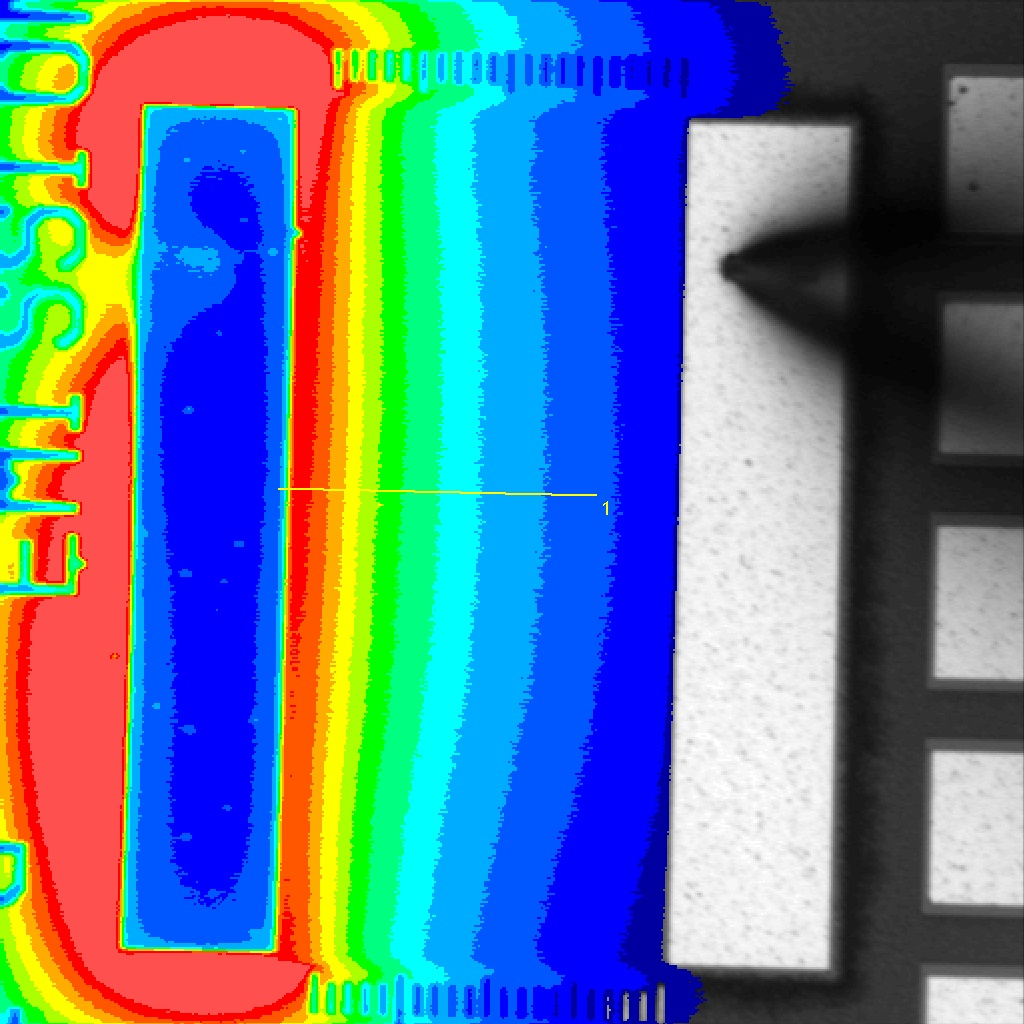
\includegraphics[scale=0.25, trim = 0cm 0cm 0cm
                            0cm,
                            clip]{./Emissionsbilder/drei/nach_Emissionsmessung_Distanz.jpg}
                            %FIXME [width=640px, height=474px]
                            \caption{selbe Diode nach der Emissionsmessung}
                        \end{figure}
                   \vspace{-1.5em}
    
                    \end{minipage}
    
                \end{tabular}
                \end{center}
                
        \vspace{2em}
        
        Die Durchlassspannung der kleineren Diode betrug $1,5 V$ bei $30 mA$
        Strom. Die Messdauer wurde auf $4s$ gestellt. Vor und nach der Messung
        wurden folgende Bilder aufgezeichnet:
        
         
         \begin{center}
                \begin{tabular}{ll}
    
                \hspace{-10em}
                    \begin{minipage}{0.6\textwidth}
    
                        \begin{figure}[H]
                            \label{fig:}
                            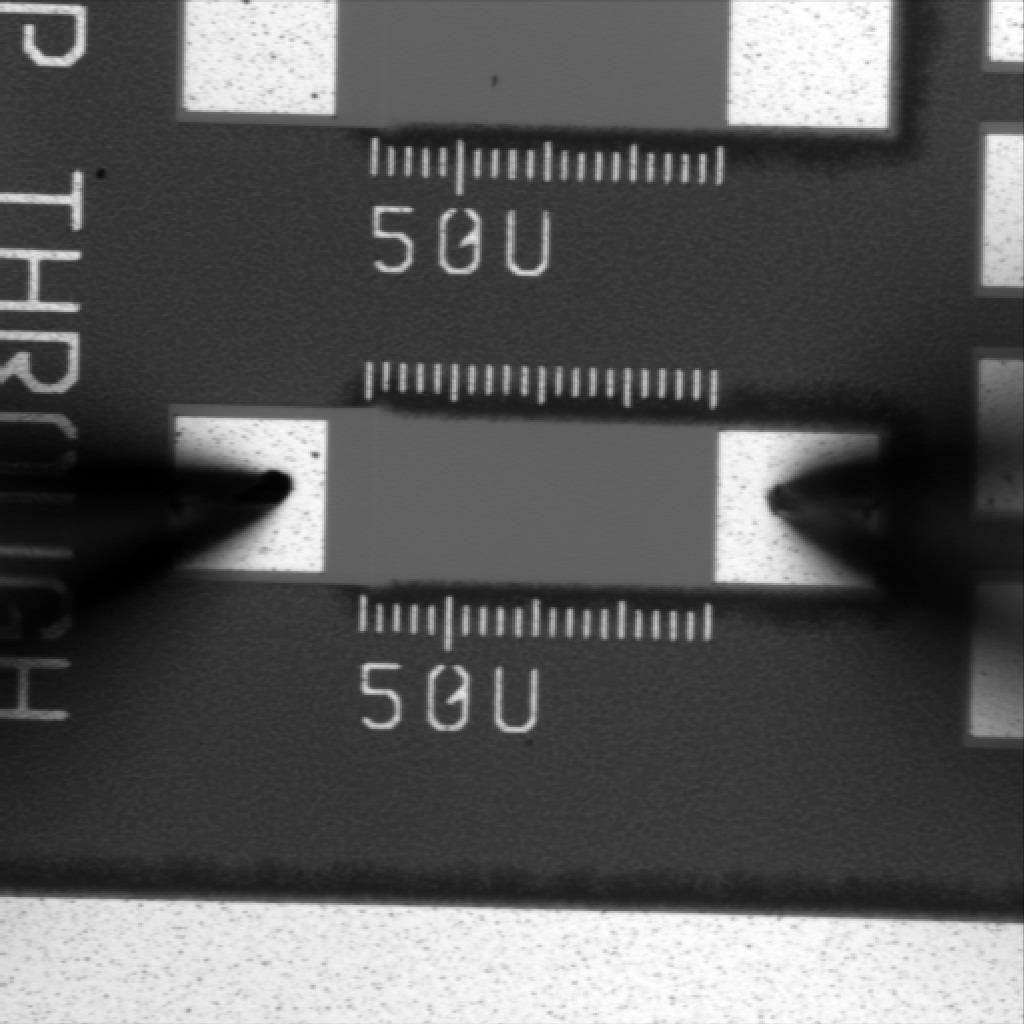
\includegraphics[scale=0.25, trim = 0cm 0cm 0cm
                            0cm,
                            clip]{./Emissionsbilder/vier/nach_Kontaktierung.jpg}
                            %FIXME [width=640px, height=474px]
                            \caption{kontaktierte Diode, Live-Bild der CCD
                            Kamera}
                        \end{figure}
    
                    \end{minipage}
                    \begin{minipage}{0.6\textwidth}
    
                         \begin{figure}[H]
                            \label{fig:}
                            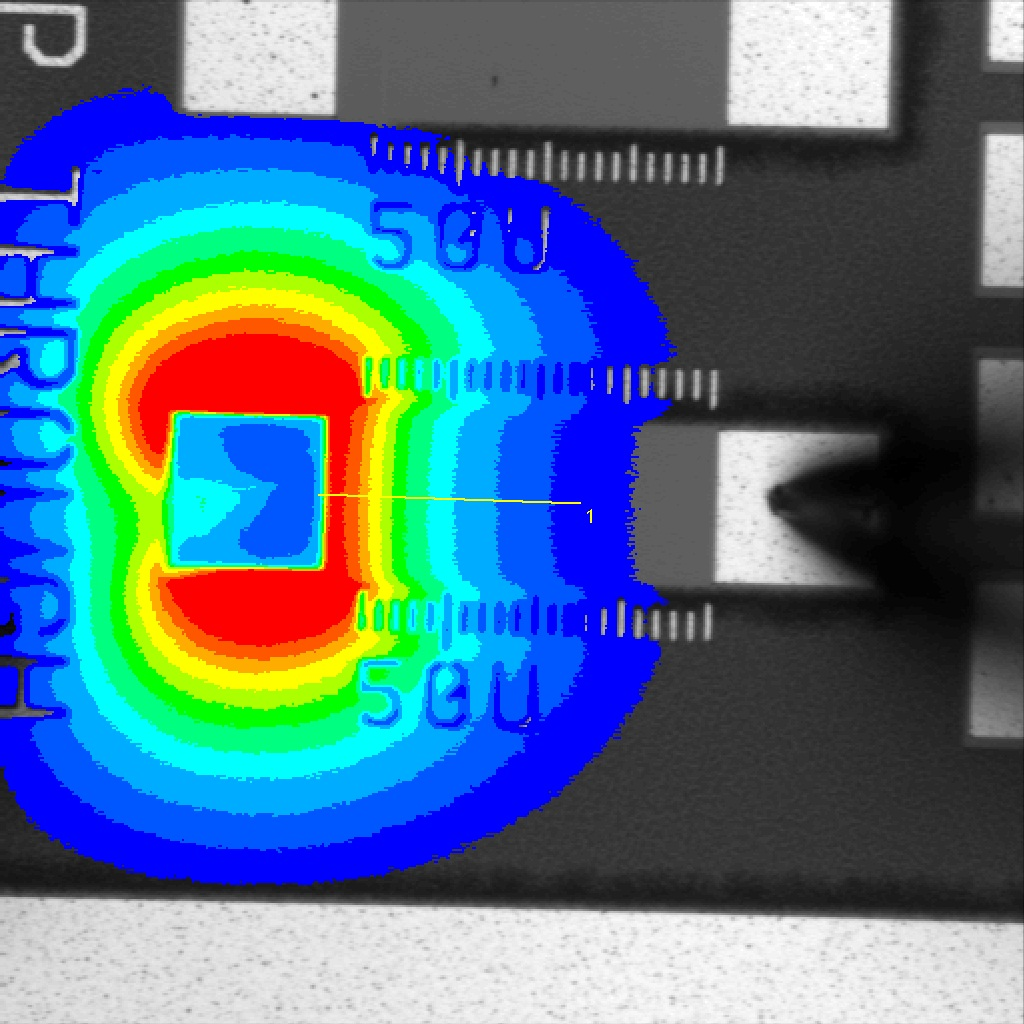
\includegraphics[scale=0.25, trim = 0cm 0cm 0cm
                            0cm,
                            clip]{./Emissionsbilder/vier/nach_Emission_Distanz.jpg}
                            %FIXME [width=640px, height=474px]
                            \caption{selbe Diode nach der Emissionsmessung}
                        \end{figure}
                   \vspace{-1.5em}
    
                    \end{minipage}
    
                \end{tabular}
                \end{center}
                
        \vspace{2em}
        
        Bislang ist nur eine Emissionsintensität zu sehen. Mithilfe der
        Phemos-Software konnte daraus ein Intensitätsprofil erstellt werden,
        woraus am Ende dann auf die Diffusionslänge zurück geschlossen werden
        kann.
        
        \end{quote}
        
        
        \section{Auswertung}
        \begin{quote}
        
        Die Phemos-Software ist in der Lage, aus der Messung eine Wertetabelle
        zu erstellen, welche die jeweilige Strahlungsintensität an dem
        betrachteten Punkt im Substrat ausgibt. Mit diesen Werten konnte Die
        Strahlungsintensität, welche den Erwartungen nach einen exponentiellen
        Abstieg aufweisen sollte, nachgebildet werden. Um zur gesuchten
        Diffusionslänge zu gelangen wird diese Kurve nun logarithmisch
        aufgetragen. Denn wenn man sich nochmal die relevante Proportionalität
        ansieht:
        
        \begin{equation*}
        \begin{split}
            I(x) \sim \ \Delta n \sim \ exp(-\frac{x}{L_n}) 
        \end{split}
        \end{equation*}
        
        dann erkennt man, dass eine Logarithmierung des Exponentialtherms nur
        das Argument übrig lässt. Daher sollte aus jeder Intensitätskurve
        eine absteigende Gerade entstehen, welche eine Steigung von $-\frac{1}{L_n}$
        besitzt. Über den Reziprokwert dieser Steigung kann man dann die
        Diffusionslänge der Dioden berechnen.
        \end{quote}
    
\end{quote} %sec Emissionsmessung

%--------------------------------------------------------------------
%--------------------------------------------------------------------


\end{document}
